%%%%%%%%%%%%%%%%%%%%%%%%%%%%%%%%%%%%%%%%%%%
%
% From a template maintained at https://github.com/jamesrobertlloyd/cbl-tikz-poster
%
% Code near the top should be fairly standard and not need to be changed
%  - except for the document class
% Code lower down is more likely to be customised
%
%%%%%%%%%%%%%%%%%%%%%%%%%%%%%%%%%%%%%%%%%%%

%%%%%%%%%%%%%%%%%%%%%%%%%%%%%%%%%%%%%%%%%%%
%
% Document class
%
% Change this if you want a different size / orientation poster etc
%
%%%%%%%%%%%%%%%%%%%%%%%%%%%%%%%%%%%%%%%%%%%

%\documentclass[portrait,a0,final]{a0poster}
\documentclass[portrait,a0,final]{a0poster}

%%%%%%%%%%%%%%%%%%%%%%%%%%%%%%%%%%%%%%%%%%%
%
% 'Basic' packages
%
% TODO - Almost certainly some are unnecessary - feel free to remove nonstandard
% packages if you think it is a good idea not to always have them
%
%%%%%%%%%%%%%%%%%%%%%%%%%%%%%%%%%%%%%%%%%%%

\usepackage{multicol}
\usepackage{color}
\usepackage{shadow}
\usepackage{morefloats}
%\usepackage{cite}
\usepackage[pdftex]{graphicx}
\usepackage{rotating}
\usepackage{amsmath, amsthm, amssymb, bm}
\DeclareMathOperator*{\argmax}{arg\,max}
\DeclareMathOperator*{\argmin}{arg\,min}
\usepackage{array}
\usepackage{nth}
\usepackage[square,numbers]{natbib}
\usepackage{booktabs}
\usepackage[table,xcdraw]{xcolor}
\usepackage{float}
%\usepackage{subfig}
%\usepackage{svg}
%\usepackage{wrapfig}
%\usepackage[a0paper,pass]{geometry}
\usepackage{array}
%%%%%%%%%%%%%%%%%%%%%%%%%%%%%%%%%%%%%%%%%%%
%
% TIKZ packages and common definitions
%
% Add extra things as per your tikz needs
%
%%%%%%%%%%%%%%%%%%%%%%%%%%%%%%%%%%%%%%%%%%%

\usepackage{picins}
\usepackage{tikz}
\usetikzlibrary{shapes.geometric,arrows,chains,matrix,positioning,scopes,calc}
\tikzstyle{mybox} = [draw=white, rectangle]

%%%%%%%%%%%%%%%%%%%%%%%%%%%%%%%%%%%%%%%%%%%
%
% myfig
%
% \myfig - replacement for \figure
% necessary, since in multicol-environment 
% \figure won't work        
%                 
%%%%%%%%%%%%%%%%%%%%%%%%%%%%%%%%%%%%%%%%%%%

\newcommand{\myfig}[3][0]{
\begin{center}
  \vspace{1.5cm}
  \includegraphics[width=#3\hsize,angle=#1]{#2}
  \nobreak\medskip
\end{center}}


\newcommand{\mydrawing}[3]{
  \vspace{0.5cm}
  \begin{center}
    \resizebox*{#2\hsize}{!}{\input{#1}}
    \label{#3}
  \end{center}
  \vspace{0.5cm}
  \stepcounter{figure}
}

%%%%%%%%%%%%%%%%%%%%%%%%%%%%%%%%%%%%%%%%%%%
%
% mycaption                
%
% \mycaption - replacement for \caption
% necessary, since in multicol-environment \figure and
% therefore \caption won't work
%
%%%%%%%%%%%%%%%%%%%%%%%%%%%%%%%%%%%%%%%%%%%

%\newcounter{figure}
\setcounter{figure}{1}
\newcommand{\mycaption}[1]{
  \vspace{0.5cm}
  \begin{center}
    {#1}
  \end{center}
  \vspace{0.5cm}
  \stepcounter{figure}
}

\setcounter{table}{1}
\newcommand{\mytablecaption}[1]{
  \vspace{0.5cm}
  \begin{center}
    \begin{quote}
        {#1}
    \end{quote}    
  \end{center}
  \vspace{1cm}
  \stepcounter{table}
}

\newcommand{\cwicaption}[1]{
  %\vspace{0.5cm}
  \begin{quote}
    {{\sc Figure} \arabic{figure}: #1}
  \end{quote}
  %\vspace{1cm}
  \stepcounter{figure}
}

\def\DD{\displaystyle}
%\DeclareMathOperator*{\argmin}{argmin}
%\DeclareMathOperator*{\argmax}{argmax}
\DeclareMathOperator*{\Var}{Var}
\DeclareMathOperator*{\Cov}{Cov}
\newcommand{\p}{{\bf q}}
\newcommand{\hp}{\hat{\bf p}}
\def\XX{{DTLR}}



%%%%%%%%%%%%%%%%%%%%%%%%%%%%%%%%%%%%%%%%%%%
%
% Some standard colours
%
%%%%%%%%%%%%%%%%%%%%%%%%%%%%%%%%%%%%%%%%%%%

\definecolor{camlightblue}{rgb}{0.601 , 0.8, 1}
\definecolor{camdarkblue}{rgb}{0, 0.203, 0.402}
\definecolor{camred}{rgb}{1, 0.203, 0}
\definecolor{camyellow}{rgb}{1, 0.8, 0}
\definecolor{lightblue}{rgb}{0, 0, 0.80}
\definecolor{white}{rgb}{1, 1, 1}
\definecolor{whiteblue}{rgb}{0.80, 0.80, 1}
\definecolor{cwired}{rgb}{0.803,0.0,0.227}

%%%%%%%%%%%%%%%%%%%%%%%%%%%%%%%%%%%%%%%%%%%
%
% Some look and feel definitions
%
%%%%%%%%%%%%%%%%%%%%%%%%%%%%%%%%%%%%%%%%%%%

\setlength{\columnsep}{0.03\textwidth}
\setlength{\columnseprule}{0.0018\textwidth}
\setlength{\parindent}{0.0cm}

%%%%%%%%%%%%%%%%%%%%%%%%%%%%%%%%%%%%%%%%%%%
%
% \mysection - replacement for \section*
% 
% Puts a pretty box around some text
% TODO - any other thoughts for what this box should look like
%
%%%%%%%%%%%%%%%%%%%%%%%%%%%%%%%%%%%%%%%%%%%

\tikzstyle{mysection} = [rectangle, 
						draw=none, 
						shade, 
						outer color=cwired,
						inner color=cwired,
						text width=0.95\columnwidth,
						text centered,
						rounded corners=20pt,
						minimum height=0.11\columnwidth]

\newcommand{\mysection}[1]
{
\begin{center}
  \begin{tikzpicture}
    \node[mysection,white] {\sffamily\bfseries\LARGE#1};
  \end{tikzpicture}
\end{center}
}



%%%%%%%%%%%%%%%%%%%%%%%%%%%%%%%%%%%%%%%%%%%
%
% Set the font
%
% TODO - Not sure what a canonical choice is - feel free to modify
%
%%%%%%%%%%%%%%%%%%%%%%%%%%%%%%%%%%%%%%%%%%%

\renewcommand{\familydefault}{cmss}
\sffamily

%%%%%%%%%%%%%%%%%%%%%%%%%%%%%%%%%%%%%%%%%%%
%
% Poster environment
%
% Centres everything and can be used to define the width of the content
%
%%%%%%%%%%%%%%%%%%%%%%%%%%%%%%%%%%%%%%%%%%%

\newenvironment{poster}{
  \begin{center}
  \begin{minipage}[c]{0.95\textwidth}
}{
  \end{minipage} 
  \end{center}
}

%%%%%%%%%%%%%%%%%%%%%%%%%%%%%%%%%%%%%%%%%%%
%
% This is probably a good place to put content specific packages and definitions
%
%%%%%%%%%%%%%%%%%%%%%%%%%%%%%%%%%%%%%%%%%%%

%%%%%%%%%%%%%%%%%%%%%%%%%%%%%%%%%%%%%%%%%%%
%
% The document environment starts here
%
%%%%%%%%%%%%%%%%%%%%%%%%%%%%%%%%%%%%%%%%%%%

\begin{document}
%%%%%%%%%%%%%%%%%%%%%%%%%%%%%%%%%%%%%%%%%%%
%
% Begin the poster environment - centres things and potentially changes the width
%
%%%%%%%%%%%%%%%%%%%%%%%%%%%%%%%%%%%%%%%%%%%

\begin{poster}

%%%%%%%%%%%%%%%%%%%%%%%%%%%%%%%%%%%%%%%%%%%
%
% Potentially add some space at the top of the poster
%
%%%%%%%%%%%%%%%%%%%%%%%%%%%%%%%%%%%%%%%%%%%

\vspace{1\baselineskip}

%%%%%%%%%%%%%%%%%%%%%%%%%%%%%%%%%%%%%%%%%%%
%
% Draw the header as a TIKZ picture
%
% Using TIKZ to allow for easy alignment
%
%%%%%%%%%%%%%%%%%%%%%%%%%%%%%%%%%%%%%%%%%%%

\begin{center}
\begin{tikzpicture}[x=0.5\textwidth]
    % Dummy nodes at edges for spacing
    % TODO - a better way?
    \node at (+1, 0) {};    
    \node at (-1, 0) {};
    % Set the size of the badges
    \def \badgeheight {0.08\textwidth}
    % Title text
    \node[inner sep=0,text width=0.8\textwidth,text centered,font=\Huge] (Title) at (-0.3,0) 
    {
        {\sffamily\veryHuge \textbf{Predicting Time Lagged Effects of Solar Activity}}\\
        {\sffamily\Huge \underline{Mandar Chandorkar}$^{1,2}$, Cyril Furthlener$^2$, 
        Bala Poduval$^3$, 
        Enrico Camporeale$^1$, 
        Michele Sebag$^2$}\\
        \vspace{-0.2\baselineskip}
        {\sffamily\large 1 Multiscale Dynamics, CWI, Amsterdam, 
        2 TAU, INRIA Paris-Saclay 
        3 UNH, New Hampshire}\\
        \vspace{-0.3\baselineskip}
        {\sffamily\LARGE www.mlspaceweather.org}
    };
    % Cambridge badge
    \node [mybox] (CWI Logo) at (-1.2, -0.4) {
        
\includegraphics[height=0.05\textwidth]{cwi-logo.png}
    };
    % CBL badge
    \node [mybox] (Inria logo) at (+0.54, -0.4) {
        
\includegraphics[height=0.05\textwidth]{inria-logo.jpg}
    };
\end{tikzpicture}
\end{center}

%%%%%%%%%%%%%%%%%%%%%%%%%%%%%%%%%%%%%%%%%%%
%
% Spacing between title and main body
%
%%%%%%%%%%%%%%%%%%%%%%%%%%%%%%%%%%%%%%%%%%%

%\vspace{.8\baselineskip}

%%%%%%%%%%%%%%%%%%%%%%%%%%%%%%%%%%%%%%%%%%%
%
% Columns environment
%
%%%%%%%%%%%%%%%%%%%%%%%%%%%%%%%%%%%%%%%%%%%



%%%%%%%%%%%%%%%%%%%%%%%%%%%%%%%%%%%%%%%%%%%
%
% Start of content
%
%%%%%%%%%%%%%%%%%%%%%%%%%%%%%%%%%%%%%%%%%%%

\large

%\begin{tabular}{lr}
%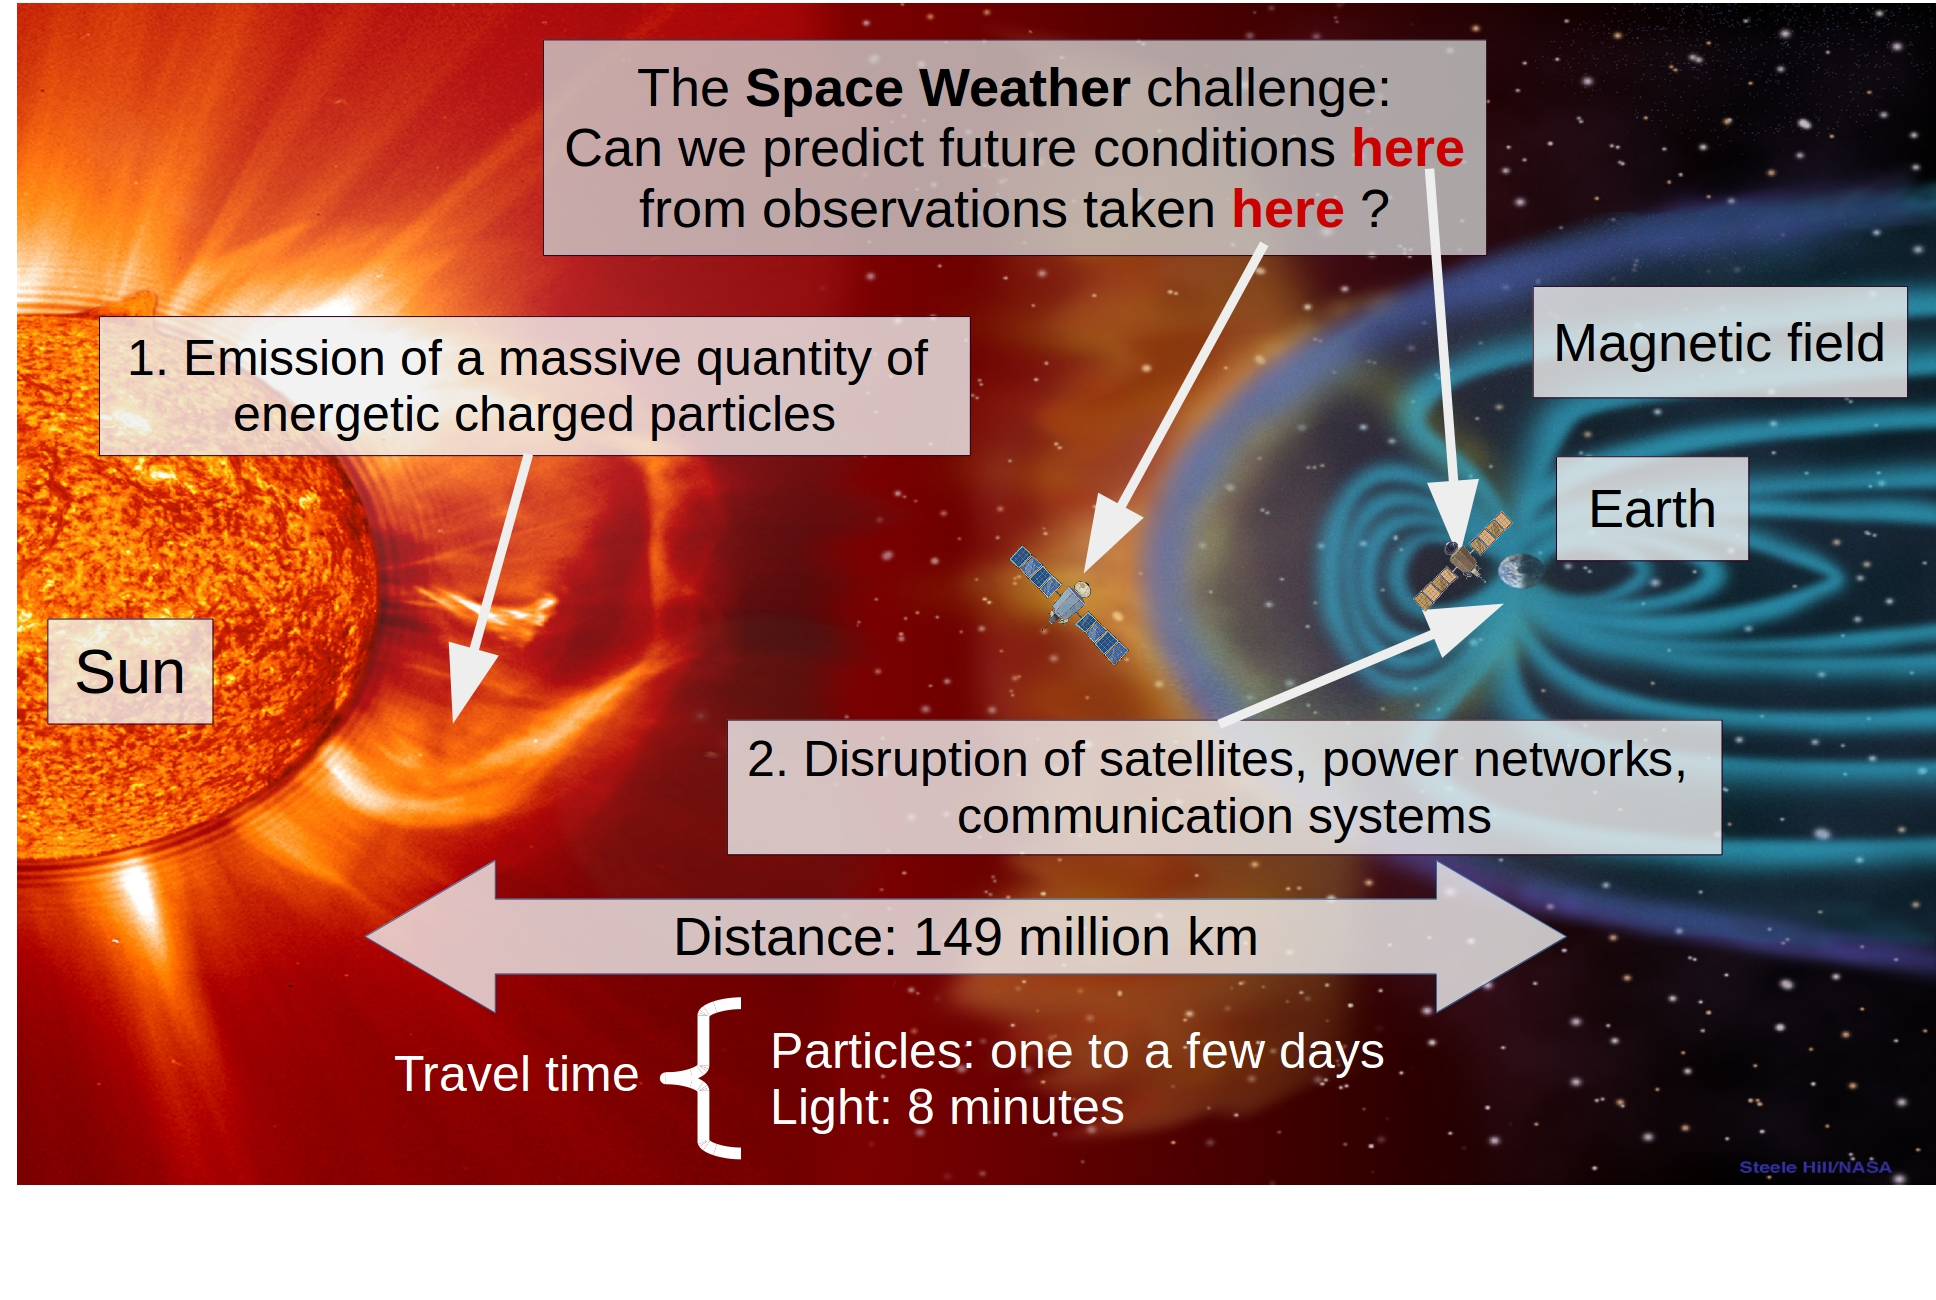
\includegraphics[width=0.48\hsize]{magnetosphere_shifted} &
%\mycaption{Space Weather Drivers and Dynamics}
%\hspace{9cm}
%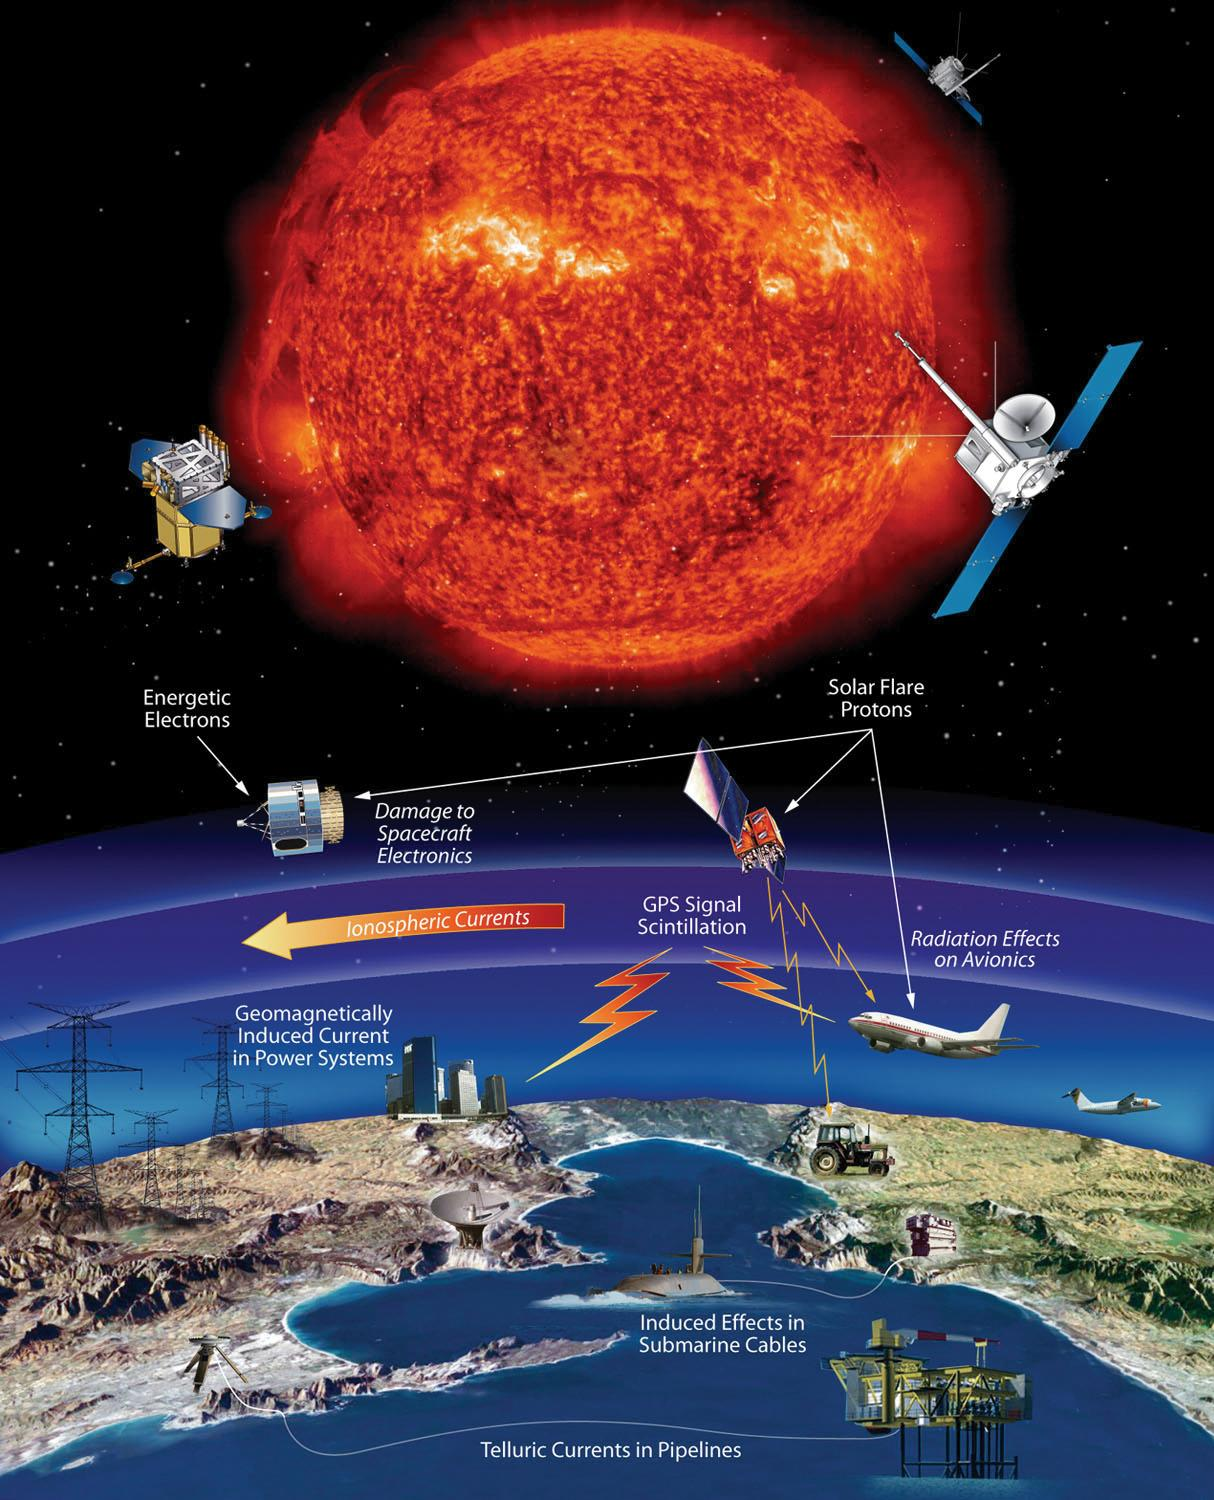
\includegraphics[width=0.28\hsize]{nasa-space-weather}\\
%\end{tabular}

\begin{multicols}{2}


\mysection{Sun-Earth System}

\myfig{parker-spiral}{0.65}

The Sun ejects charged energetic particles, known as the \emph{solar wind}, into the surrounding space. 
Depending on the nature of activity on the Sun, its effects are observed near the Earth after some time delay, 
which is variable and uncertain.

\vspace{0.5\baselineskip}
\mysection{Dynamic Time-Lag Regression}
\myfig{GrangerCausalityIllustration}{0.65}

Learning the the time delay between causes and effects, from data, is an important and challenging problem. We call this problem 
\emph{Dynamic Time Lag Regression} (\XX) and formulate it as follows.
%\vfill
%\columnbreak

\begin{enumerate}
\item \textbf{Inputs}: Two time series, the causes $x(t)$ and the observed effects $y(t)$
\item \textbf{Outputs}: A function $f: \mathcal{X}  \rightarrow \mathbb{R}$ which maps each input pattern 
  $x(t_1)$ to an output $y(t_2)$, and $g:\mathcal{X}  \rightarrow \mathbb{R}^{+}$ which maps the time delay 
  between the input and output patterns $t_2 = t_1 + g(x(t_1))$.
\end{enumerate}

\begin{align}
y(t + \Delta(t)) & = f[x(t)]\label{eq:pb1}\\
\Delta(t) & = g[x(t)]\label{eq:pb2} 
\end{align}

\mysection{Proposed Solution}

Define for every time step $t$, a time window $[t+\ell, t+\ell+h)$. 
\vspace{0.4\baselineskip}

\textbf{Inputs}: Time series $x(t) \in \mathbb{R}^{n}$ \vspace{0.5\baselineskip}

\textbf{Model Outputs}: 
\begin{enumerate}
\item Targets $[\hat{y}(t+\ell), \dots, \hat{y}(t+\ell+h-1)]$
\item Time Lag Probabilities $[\hat{p}(t+\ell), \dots, \hat{p}(t+\ell+h-1)], \ \sum^{h-1}_{i = 0}{\hat{p}_{i}} = 1$
\end{enumerate}

\vspace{0.4\baselineskip}

\textbf{Predictions}: For an input $x(t)$, predict the target $\hat{y}(t + \ell + i^{*})$ corresponding to the most probable propagation time $i^{*} = \argmin_{i}{\hat{p}_i(x(t))}$

\vspace{0.4\baselineskip}

\textbf{Architecture}: The proposed model architecture takes the form of a neural network model as seen below.
\mydrawing{archi.tex}{0.6}{fig:NN}

\textbf{Model Training}: In order to build time lag based models, we must devise an objective/loss function which favours.

\begin{enumerate}
    \item Accurate predictions for time window: $\hat{y}(t+\ell), \dots, \hat{y}(t+\ell+h-1)$
    \item Learning the time lag structure by penalising $\hat{p}(t+\ell), \dots, \hat{p}(t+\ell+h-1)$.
\end{enumerate}


%
\begin{equation}\label{eq:LL}
  {\cal L}\bigl[ {\bf x, y};\hat {\bf y},\hat {\bf p},\sigma,{\bf \alpha}] = 
  -\vert T\vert\log(\sigma)-\frac{1}{n_m}\sum_m\Bigl[
    \sum_{i \in T}\frac{1}{2\sigma^2}\bigl(y_{m+i}-\hat y_i(x_m)\bigr)^2 - 
    \log\bigl(Z_m(\hat {\bf y},\hat {\bf p},\sigma,{\bf \alpha})\bigr)\Bigr],
\end{equation}
%
with $n_m$ the number of data points and partition term $Z_m$ given as:
\[
  Z_m(\hat {\bf y},\hat {\bf p},\sigma,{\bf \alpha}) = \sum_{i \in T}\hat p_i(x_m)\exp\Bigl(
    - \frac{1}{2\sigma^2}\sum_{j\in T}\alpha_{ji}\bigl(y_{m+j}-\hat y_j(x_m)\bigr)^2 
    + \frac{1}{2}\sum_{j\in T}\log(1+\alpha_{ji})\Bigr).
\]


\vspace{0.5\baselineskip}

\mysection{Experiments}

\textbf{Input Data} 

\begin{itemize}
  \item Magnetic flux-tube expansion $\log \mathbf{f}_S$ and source surface field 
  $\mathbf{B}_{ss}$. Both computed from GONG synoptic maps using the 
  \emph{Current-Sheet Source Surface} (CSSS) \citep{csss} model.
  \item $\Phi$, the Carrington longitude of the computed of each time-stamped $\mathbf{f}_S$.
  \item Sun spot number $SSN$ and $F_{10.7}$ indices from OMNI.
\end{itemize} 

\myfig{test_scatter_v}{0.5}

\mycaption{\textbf{Problem I}: Output vs Propagation time relationship}


\begin{center}
  \label{tab:results_reiss}
  \centering
  \begin{tabular}{ l l l }
  \hline
  Model &  M.A.E & R.M.S.E \\
  \hline
  \XX & $54.41$ & $66.22$ \\
  Fixed Lag Baseline & $67.33$ & $80.39$ \\
  WS & $74.09$ & $85.27$ \\
  DCHB & $83.83$ & $103.43$ \\
  WSA & $68.54$ & $82.62$ \\
  Ensemble Median (WS)   & $71.52$ & $83.36$ \\
  Ensemble Median (DCHB) & $78.27$ & $100.04$ \\
  Ensemble Median (WSA)  & $62.24$ & $74.86$ \\
  Persistence (4 days)   & $130.48$ & $161.99$ \\
  Persistence (27 days)  & $66.54$ & $78.86$ \\
  \hline
  \end{tabular}
  \mycaption{
    Performance Comparison on CR $2077$: \XX \ , 
    Fixed Lag Base Line vs \citet{Reiss_2019}
  }
\end{center}


\bibliographystyle{rusnat}
\bibliography{sample}

%\vspace{\baselineskip}
%\vspace{.5\baselineskip}
%Ref: Chandorkar, Camporeale, Wing \emph{Gaussian Processes Autoregressive Models for Forecasting the Disturbance Storm Time Index}

\end{multicols}

\end{poster}

\end{document}
